\subsection{Desarrollo de servidor web}

\paragraph{Introducción}
Este sección tiene como objetivo mostrar los puntos clave en el desarrollo de un servidor con una Arquitectura de Orientada a Microservicios, dicho servidor fue utilizado en el presente trabajo para realizar las tareas de comunicación con una Aplicación Móvil, ejecución de algoritmos de ordenamiento y la conexión con un SGBD el cuál persistirá toda la información generada por el sistema. \\

A continuación, se mencionarán los componentes más importantes de dicha arquitectura así como las tecnologías que se utilizaron para implementar estos componentes, se dará un breve ejemplo de código y finalmente se mostrarán algunos de los resultados que se obtuvieron. \\

\paragraph{Objetivos Microservicios}
Una Arquitectura de Microservicios posee ciertas características que deben de ser cumplidas para garantizar el correcto funcionamiento del sistema, cada una de estas características permite cumplir con un objetivo, a continuación se hace una lista de las características principales que se desea tenga una arquitectura básica:

\begin{itemize}
	\item \textbf{Bounded Context:} Es la acción de dividir nuestro sistema en diferentes servicios, cada uno de estos deberá tener la granularidad correcta y además deberán ser expuestos al exterior (normalmente a través de un Web services) además, dichos podrán comunicarse entre sí.
	\item \textbf{Configuration Management:} Permite almacenar todas las configuraciones necesarias para los servidores en un repositorio centralizado, de manera tal, que estas configuraciones puedan ser expuestas y consultadas por nuestros microservicios, esto permite un mejor mantenimiento de las configuraciones del sistema.
	\item \textbf{Dynamic Scale Up/Down:} Esta característica permite realizar dos operaciones de suma importancia dentro de esta arquitectura como lo son:
	\begin{itemize}
		\item Registro de servicios: Todas las instancias de nuestro servidores deberán registrar en un Name Server, el cuál es análogo a un directorio telefónico que posee los nombres y las direcciones de todos los servidores activos.
		\item Descubrimiento de servicios: La arquitectura debe de poder revisar de manera dinámica todas las instancias que se encuentren activas en cierto punto del tiempo.
		\item Load Balancing: Permite distribuir toda la carga de peticiones a través de todas las instancias activas de nuestros Microservicios.
	\end{itemize}
	\item \textbf{Visibility and Monitoring:} Permite conocer el estado actual de nuestros Microservicios esto con el fin de monitorear el uso de recursos a través de todos los componentes de nuestro servidor así como proporcionar datos analíticos y de seguridad.
	\item \textbf{Fault Tolerance:} Si uno de nuestros servidores sufre algún percance podemos tener una infraestructura que impida que este error se propague.
\end{itemize}


\paragraph{Componentes de una Arquitectura Orientada a Microservicios}
Para poder cumplir con las características antes mencionadas es necesario implementar un conjunto de componentes (cada uno de estos hace uso de una tecnología en específico) dentro de nuestra arquitectura, a continuación se listan los componentes que fueron utilizados para este trabajo:

\begin{itemize}
	\item Microservicios expuestos a través del protocolo REST.
	\item Tecnologías para el desarrollo en Cloud.
	\begin{itemize}
		\item API Gateway
		\item Load Balancer
		\item Naming Server
		\item Configuration Server
		\item Tracing Server
	\end{itemize}
\end{itemize}

\paragraph{Tecnologías utilizadas}
Como ya se mencionó, cada uno de los componentes antes mencionados implementa una tecnología diferente para poder llevar a cabo sun funcionalidad. El presente trabajo utilizó los siguientes frameworks de desarrollo para la implementación de la Arquitectura de Microservicios.

\begin{itemize}
\item \textbf{Spring Framework} Spring es un framework para el desarrollo de aplicaciones que posee un contenedor de Inversión de Control de código abierto para la plataforma Java.

\item \textbf{Spring Cloud} Spring Cloud es un framework para la construcción de aplicaciones en la nube. El framework facilita el desarrollo de aplicaciones al proporcionar soluciones a muchos de los problemas comunes que se enfrentan al trabajar en un entorno distribuido.

Las aplicaciones que se ejecutan con la arquitectura de microservicios tienen como objetivo simplificar el desarrollo, la implementación y el mantenimiento. La naturaleza descompuesta de la aplicación permite a los desarrolladores enfocarse en un problema a la vez.	
\item \textbf{Netflix OSS} Es un framework que contiene un conjunto de tecnologías de tipo open source para el desarrollo de sistemas distribuidos, concretamente el desarrollo de microservicios, que han sido puestas a nuestra disposición por la empresa Netflix.

\item \textbf{Spring Cloud Netflix} Spring Cloud Netflix proporciona integraciones de Netflix OSS para las aplicaciones Spring Boot a través de la configuración automática y el enlace con Spring Environment y otros lenguajes de modelos de programación de Spring. Con unas pocas anotaciones simples, puede habilitar y configurar rápidamente los patrones comunes dentro de su aplicación y construir grandes sistemas distribuidos con componentes de Netflix probados en la batalla.
\end{itemize}	
\paragraph{Descripción de la tecnologías} Una vez que se han mencionado los frameworks a utilizar, es momento de pasar a una descripción más detallada de como se construyeron cada uno de los componentes antes mencionados haciendo uso de las tecnologías pertinentes. A continuación, se muestra una imágen con una diagrama general de las tecnolgías usadas, así como su interconexión.

\begin{figure}[H]
	\centering
	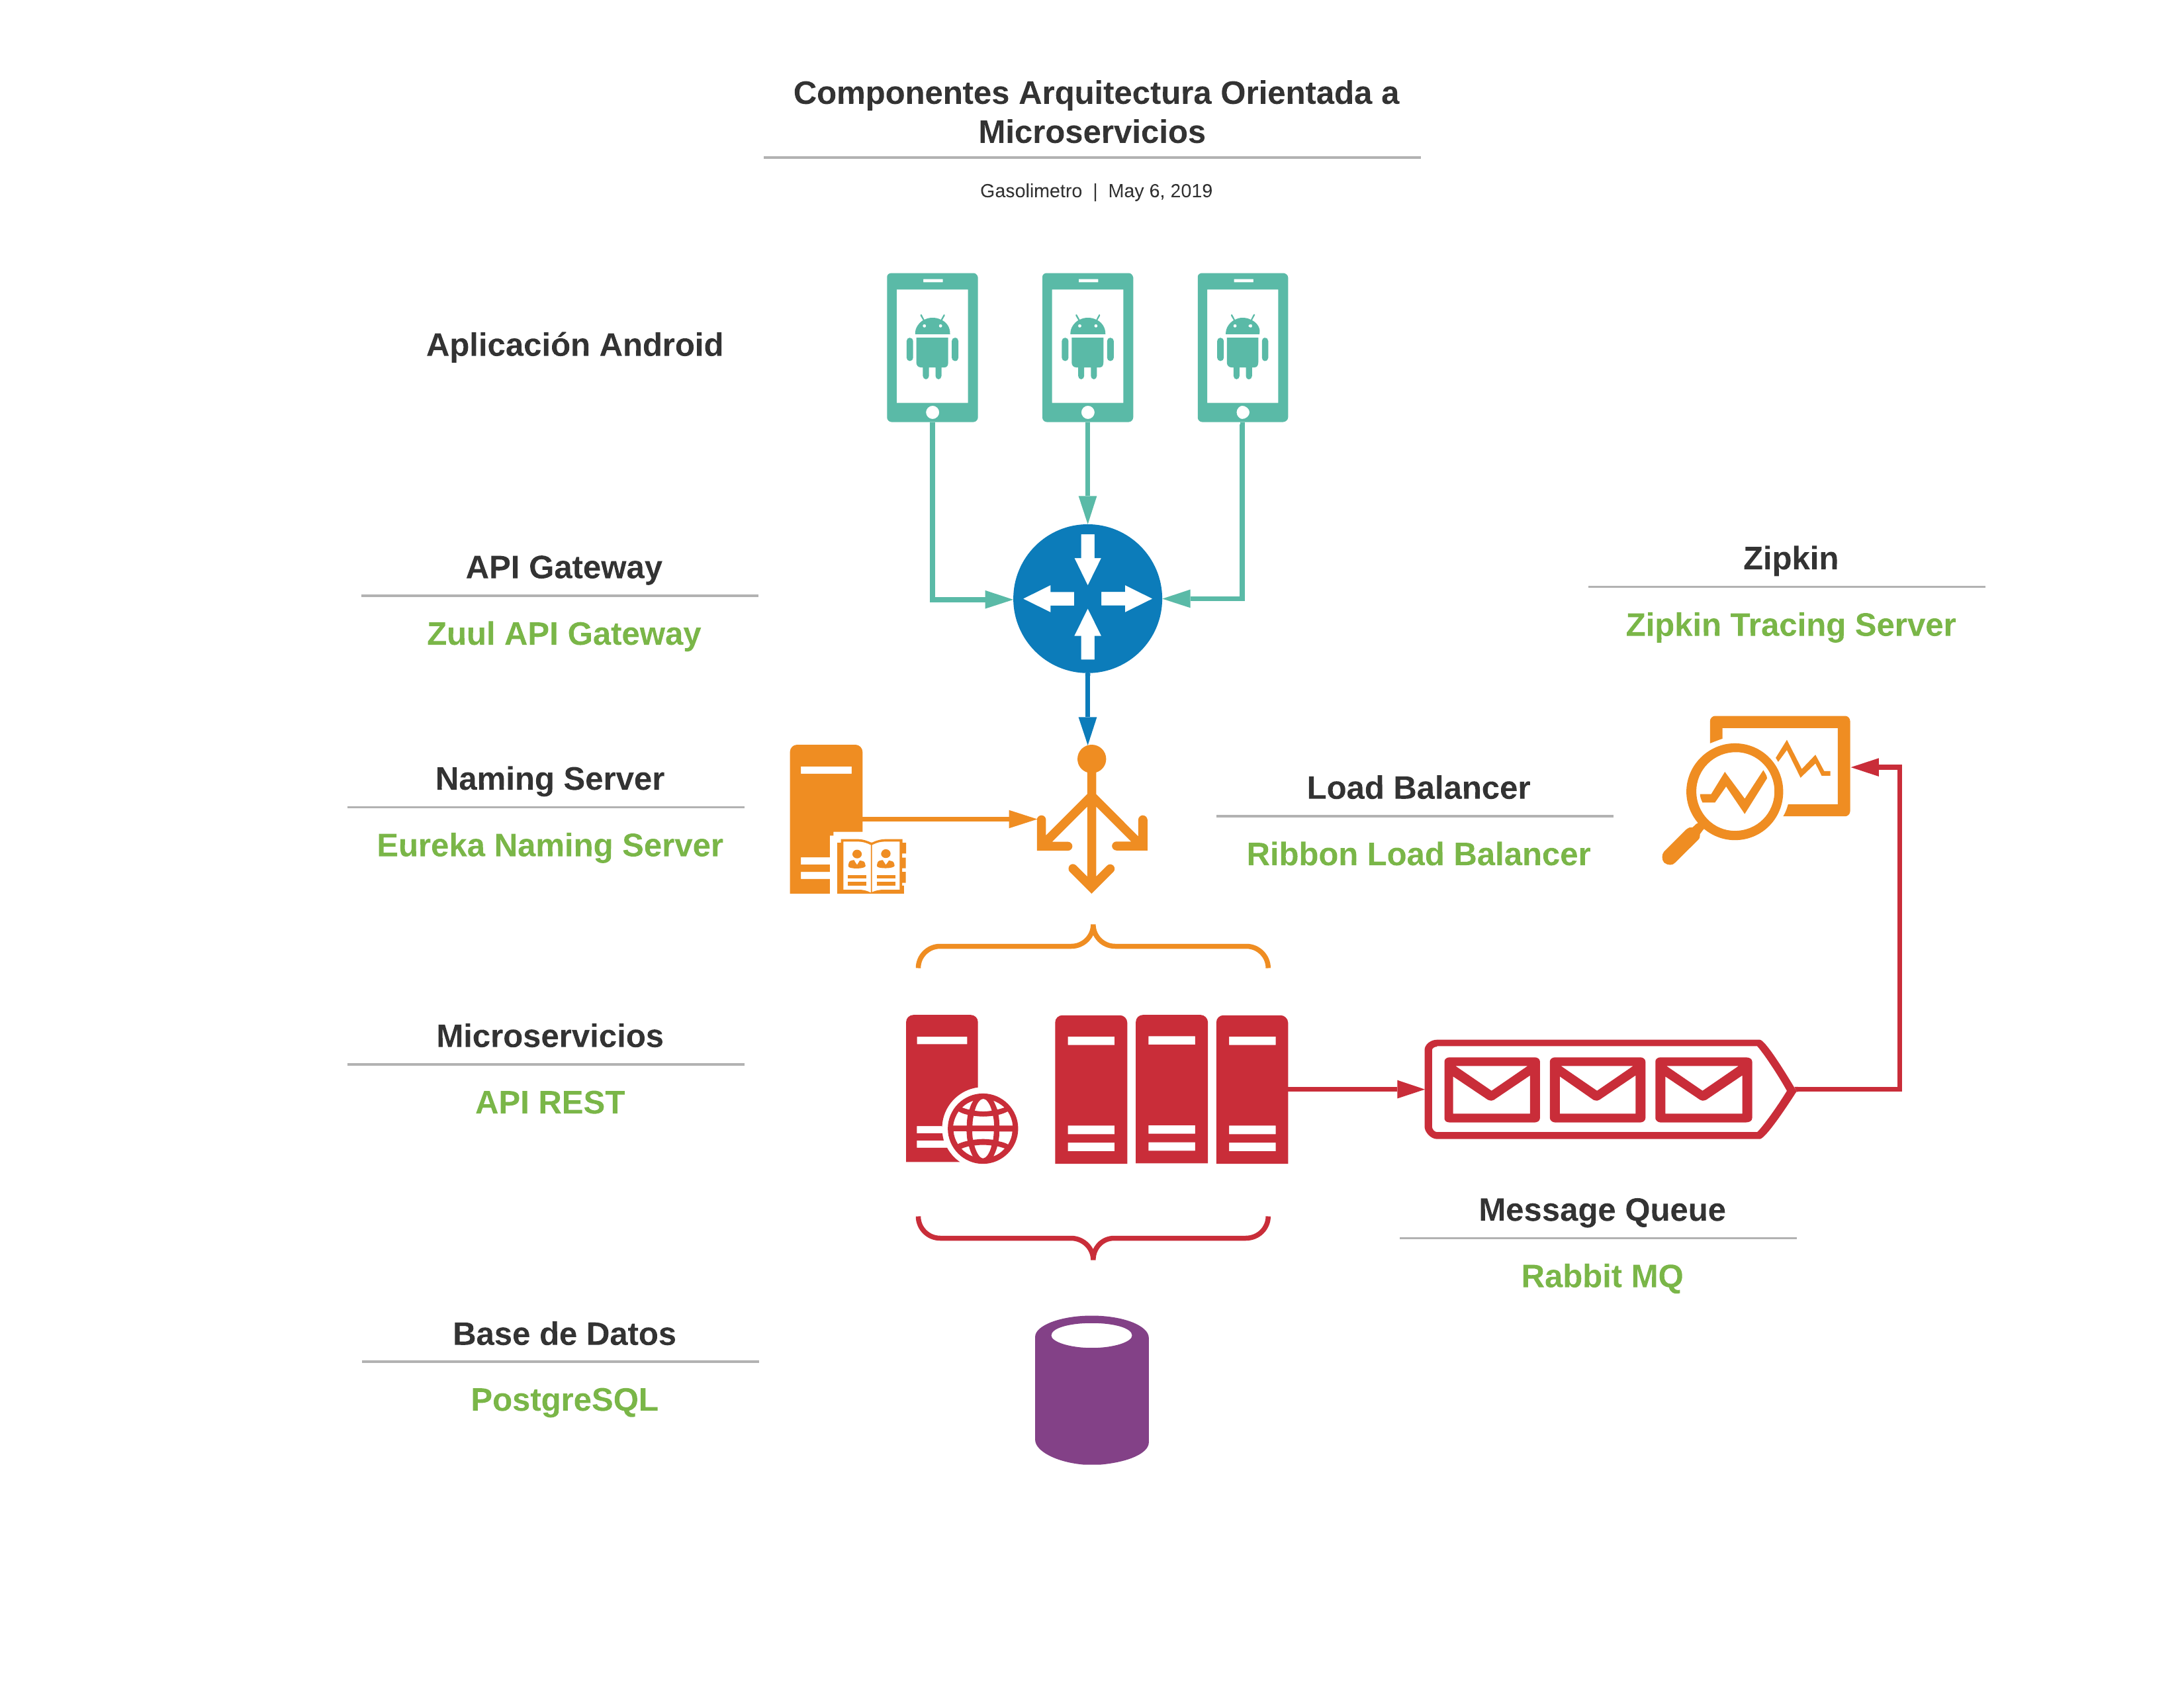
\includegraphics[scale=.14]{Capitulo5/software/submodulos/servidor/images/arquitectura.png}
	\caption{Arquitectura de un Servidor Orientado a Microservicios utilizando Spring Framework 8}
	\label{fig:arquitecura_servidor}
\end{figure}

\paragraph{Creando un Microservicio}

